\chapter{Kontraktion in Sichtbarkeitsgraphen}\label{chapter:kontraktion}

Die zuvor beschriebene Kontraktion von Knoten und Graphen ist bei Graphen mit hohem durchschnittlichen Knotengrad, wie zum Beispiel Sichtbarkeitsgraphen, deutlich rechenintensiver als bei Graphen mit geringeren Knotengrad, wie etwa Straßengraphen.
Für die Knoten-Kontraktion muss für jeden Vorgänger eine Dijkstra-Suche durchgeführt werden, und für jedes Paar aus Vorgänger und Nachfolger ist zu prüfen, ob eine Abkürzung eingefügt werden muss.
Ein hoher Knotengrad bedeutet somit viele Dijkstra-Suchen und $\abs{\text{Vorgänger}} \cdot \abs{\text{Nachfolger}}$ viele Vergleiche, ob eine Abkürzung notwendig ist.

Bei der Bottom-Up-Kontraktion wird die Kontraktion potenziell mehrfach simuliert, bevor sie wirklich ausgeführt wird:
Beim Lazy-Popping werden die Knoten oft nicht kontraktiert, sondern mit aktualisiertem Heuristik-Wert in die Warteschlange zurückgeschoben, da durch viele Nachbarn die Wahrscheinlichkeit dafür steigt, dass sich die Knoten-Differenz verändert hat.
Beim Neighbor-Update sind jeweils sehr viele Nachbarn zu aktualisieren.

Um Graphen mit hohen Knotengraden schneller zu kontrahieren, ist es entscheidend, die Kontraktion einzelner Knoten zu beschleunigen und eine effiziente sowie effizient erstellbare Reihenfolge der Kontraktionen zu finden.
Auch die zur Repräsentation von Graphen verwendeten Datenstrukturen sollten optimiert werden, sodass das Finden von Nachbarn sowie das Einfügen und Löschen von Kanten effizient und parallel möglich ist.

\section{Kontraktion mit Heuristik}

Anstelle einer rechenintensiven Dijkstra-Suche in $G$ pro Vorgänger kann eine Heuristik pro Paar aus Vorgänger und Nachfolger eine obere Schranke für den Abstand geben.
Eine Kante als Abkürzung wird dann eingefügt, wenn ihre Länge kleiner oder gleich der berechneten oberen Schranke ist.
Damit dies für die Kontraktion eines einzelnen Knotens effizienter ist, muss die Ermittlung der Heuristikwerte für alle Paare aus Vorgänger und Nachfolger schneller sein als die Dijkstra-Suchen und die anschließenden Abfragen der Distanzen der Dijkstra-Suche.
Damit die Kontraktion des gesamten Graphen effizienter ist, müssen die Folgekosten unnötigerweise eingefügter Kanten geringer sein als der Zeitgewinn durch den Einsatz der Heuristik.

\subsection{Triviale Heuristik}

Die \emph{Triviale Heuristik} setzt die obere Schranke für jedes Knotenpaar auf $\infty$.
Dies bedeutet, dass für jedes Paar aus Vorgänger und Nachfolger, unabhängig von der tatsächlichen Distanz, eine Kante als Abkürzung eingefügt wird.
Unter der Annahme, dass in Graphen mit sehr hohem Knotengrad fast alle Nachbarn bereits mit einer Kante verbunden sind, könnte der Anteil der unnötig eingefügten Abkürzungen im Vergleich zu den notwendigen vernachlässigbar sein.

\subsection{Vereinfachter Graph}

Sei $G = (V, E)$ der zu kontrahierende Graph.
Lässt sich zu $G$ effizient ein vereinfachter Graph $G' = (V', E')$ mit $V \subset V'$ und $\forall s, t \in V \colon {spd}_{G'} (s, t) \geq {spd}_{G} (s, t)$ konstruieren, so kann dieser zur Berechnung der oberen Schranke verwendet werden, etwa indem die Dijkstra-Suchen auf ihm ausgeführt werden.
Alternativ kann aus $G'$ auch ein Contracted- oder Hub-Graph erzeugt werden, womit die obere Schranke dann für jedes Vorgänger-Nachfolger-Paar einzeln berechnet wird.

Für Graphen in der euklidischen Ebene existieren Algorithmen, wie etwa die Delaunay-Triangulierung, die es ermöglichen, leicht einen vereinfachten Graphen zu erstellen.

\subsection{Dreiecksungleichung}

Ähnlich zu ALT\cite{goldberg2005computing} kann eine Menge \emph{Hubs} berechnet werden, welche mittels der Dreiecksungleichung eine obere Schranke des Abstands zweier Knoten angeben können.
Ein Hub ist hierbei ein Knoten $h \in V$, für den die Distanzen zu und von allen Knoten bekannt sind.
Die obere Schranke des Abstandes zweier Knoten $s, t \in V$ kann dann durch ${spd}_G (s, h) + {spd}_G (h, t)$ berechnet werden.
Liegt $h$ dabei auf einem kürzesten Pfad von $s$ nach $t$, so entspricht der Wert sogar genau dem Abstand.
Die obere Schranke über mehrere Hubs wird durch die Wahl der kleinsten oberen Schranken bestimmt.
Es reicht sogar, eine obere Schranke zu finden, die kleiner ist als die potenzielle Abkürzung; in diesem Fall kann die Kante keine optimale Abkürzung sein, und die Überprüfung kann abgebrochen werden.

\begin{figure}[h!]
    \centering
    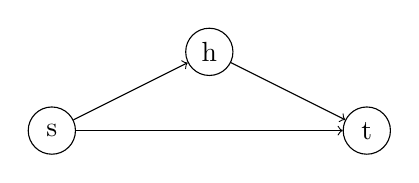
\begin{tikzpicture}[scale=1]
        \node[circle, draw, minimum size=0.6cm, inner sep=0pt] at (0.0, 0.0)  (s)    {s};
        \node[circle, draw, minimum size=0.6cm, inner sep=0pt] at (4.0, 0.0)  (t)    {t};
        \node[circle, draw, minimum size=0.6cm, inner sep=0pt] at (2.0, 1.0)  (h)    {h};
        \draw[->]  (s) edge node {} (t);
        \draw[->]  (s) edge node {} (h);
        \draw[->]  (h) edge node {} (t);
    \end{tikzpicture}

    \caption{Beispiel eines Hubs}
\end{figure}

Die Hubs können dabei über die Berechnung eines Hitting-Sets bestimmt werden.
Durch die Auswahl von Hubs auf diese Art steigt die Genauigkeit der oberen Schranken mit der Hop-Länge der kürzesten Pfade, da die Wahrscheinlichkeit, dass diese durch einen Hub getroffen wird, steigt.
Durch mehr Hubs steigt allerdings auch der Zeitbedarf der Berechnung der oberen Schranke.

\subsection{Kombination mehrerer oberer Schranken}
Sind für einen Graphen mehrere Heuristiken bekannt, so kann für eine potenzielle Abkürzung aus allen oberen Schranken die kleinste ausgewählt werden.
Dies ist besonders dann sinnvoll, wenn die Heuristiken jeweils eine Teilmenge aller Knotenpaare \emph{gut} abdecken.
Insbesondere die Kombination von Dreiecksungleichung und vereinfachtem Graph ist hierbei vielversprechend, unter der Annahme, dass die erste für große und die zweite für kleine Hop-Abstände gute obere Schranken liefert.

\section{Datenstruktur}

Werden auf dem zu kontrahierenden Graphen keine Dijkstra-Suchen durchgeführt, ändern sich die Anforderungen an die zur Repräsentation des Graphen verwendete Datenstruktur.
Während für Dijkstra-Suchen vor allem das schnelle Auffinden ausgehender Kanten wichtig ist, sind bei der Kontraktion mit oberer Schranke das schnelle Auffinden einer $s$-$t$-Kante sowie das Isolieren eines Knotens wichtig.

Die Knoten-Kontraktion erfolgt hierbei in zwei Schritten.
Im ersten Schritt werden alle einzufügenden Kanten berechnet, wobei zwischen neuen und zu aktualisierenden Kanten unterschieden wird.
Eine Kante wird aktualisiert, wenn bereits eine Kante mit höherem Kantengewicht existiert.
Das Abfragen des Kantengewichts sollte daher unmittelbar, ohne eine Suche, möglich sein.
Das Aktualisieren von Kanten kann bei den meisten Datenstrukturen parallel erfolgen, während das Einfügen neuer Kanten nur eingeschränkt parallelisierbar ist.
Im zweiten Schritt wird der Graph modifiziert, indem die neuen Kanten eingefügt und der zu kontrahierende Knoten isoliert wird.

Es empfiehlt sich daher, pro Knoten eine HashMap zu verwenden, die den Nachfolgern das entsprechende Kantengewicht zuweist.
Die effiziente Überprüfung, ob eine Kante bereits vorhanden ist, lässt sich dadurch realisieren, und für jeden Vorgänger eines zu kontrahierenden Knotens können parallel Kanten in die jeweilige HashMap eingefügt werden.
